% ============================================================================
%  WireClaim — the organisers' "short write-up of your approach".
%  Team "Bin busy", QuantCo Claim to Fame, Munich Agentic Hackathon 2026.
%  Build:  latexmk -pdf writeup.tex      (or: pdflatex writeup.tex  x2)
% ============================================================================
\documentclass[10pt,a4paper,twocolumn]{article}

\usepackage[T1]{fontenc}
\usepackage[utf8]{inputenc}
\usepackage[margin=1.55cm,columnsep=0.75cm]{geometry}
\usepackage{amsmath,amssymb}
\usepackage{booktabs}
\usepackage{graphicx}
\usepackage{microtype}
\usepackage{xcolor}
\usepackage{eurosym}
\usepackage{multicol}
\usepackage[hidelinks]{hyperref}
\usepackage{enumitem}
\usepackage{caption}

\definecolor{accent}{HTML}{9A6B00}
\definecolor{good}{HTML}{2F6B3A}
\definecolor{bad}{HTML}{9C3323}
\definecolor{rule}{HTML}{BFBFBF}

% Compact section headings without titlesec (BasicTeX does not ship it).
\makeatletter
\renewcommand\section{\@startsection{section}{1}{\z@}%
  {1.1ex \@plus .3ex \@minus .2ex}{0.5ex \@plus .2ex}%
  {\normalfont\normalsize\bfseries}}
\renewcommand\subsection{\@startsection{subsection}{2}{\z@}%
  {0.9ex \@plus .2ex \@minus .1ex}{0.3ex \@plus .1ex}%
  {\normalfont\small\bfseries}}
\renewcommand{\thesection}{\textcolor{accent}{\arabic{section}}}
\makeatother
\setlist[itemize]{leftmargin=1.1em,itemsep=0.22ex,topsep=0.35ex,parsep=0pt}
\captionsetup{font=footnotesize,labelfont=bf,skip=3pt}
\setlength{\parskip}{0.25ex}
\pagestyle{empty}

% notation shorthands
\newcommand{\charge}{a}
\newcommand{\limitv}{b}
\newcommand{\fair}{t}
\newcommand{\est}{\hat{t}}

\begin{document}

\twocolumn[%
\begin{@twocolumnfalse}
\begin{center}
{\LARGE\bfseries WireClaim}

\vspace{0.4em}
{\large Recovering latent fair values from settled transactions}

{\large in a repeated two-sided pricing game}

\vspace{0.7em}
{\normalsize Team \textbf{Bin busy} \;\textbullet\; QuantCo \emph{Claim to Fame} (Track 1)
\;\textbullet\; Munich Agentic Hackathon, 22--23 August 2026}

\vspace{1.0em}
\begin{minipage}{0.86\textwidth}
\small
\textbf{Abstract.} Each of 100 Games releases an insurance policy, a damage description and a
price-less invoice; within 60 seconds we must submit, per Line Item, a Charge $\charge$ and an
acceptance Limit $\limitv$ against a hidden fair value $\fair$. We show (i) that the payoff table
makes the Charge a \emph{cliff} rather than a slope, so the optimal Charge sits strictly below the
estimate; (ii) that $\fair$ is \emph{exactly recoverable} after settlement from the published
transaction log, which converts every design question into a measurement; and (iii) that under
this instrument the entire remaining gap to optimal play is estimation error, not strategy. We
report a climb from last place (17th of 17) to 5th, the second-best per-Game rate in the field
over the last twenty Games, and the second-best risk-adjusted return, with two losing Games in
twenty.
\end{minipage}

\vspace{1.2em}
\end{center}
\end{@twocolumnfalse}
]

\section{The game}

Per ordered pair (issuer $H$, reviewer $I$) and Line Item, with hidden fair value $\fair$ and
hidden cap $c \ge \max(4\fair, 2000)$:
\begin{equation}
\pi_H=\!
\begin{cases}
\charge & \charge \le \fair \quad\text{(any } \limitv)\\
\min(\charge,c) & \charge > \fair,\ \charge \le \limitv\\
0 & \charge > \fair,\ \charge > \limitv
\end{cases}
\label{eq:issuer}
\end{equation}
\vspace{-1.1em}
\begin{equation}
\pi_I=\!
\begin{cases}
-\charge & \charge \le \fair,\ \charge \le \limitv\\
\mathbf{-1.5\,\charge} & \charge \le \fair,\ \charge > \limitv\\
-\min(\charge,c) & \charge > \fair,\ \charge \le \limitv\\
0 & \charge > \fair,\ \charge > \limitv
\end{cases}
\label{eq:reviewer}
\end{equation}

\noindent
Row~1 of \eqref{eq:issuer} is the clause that decides the game: \textbf{if the Charge is fair the
issuer is paid whatever the reviewer does.} A fair Charge is therefore owed by all $N=16$
opponents; an Overcharge is paid only by those few whose Limit happens to exceed it. Measured on
Game~62: \textbf{16 payers versus 3}. Score is $\text{net}=\sum \pi_H + \sum \pi_I$ over all
ordered pairs and all Games, with Games 81--100 weighted $3\times$.

\section{The Charge is a cliff}

Let $F$ be the posterior CDF of $\fair$ and let $q(\charge)$ be the fraction of opponents whose
Limit admits $\charge$. Expected issuer income per opponent is
\begin{equation}
R(\charge)=\charge\big[\,\underbrace{1-F(\charge)}_{\text{fair: everyone pays}}
+\;\underbrace{F(\charge)\,q(\charge)}_{\text{overcharge: few pay}}\big].
\end{equation}
Empirically $q$ collapses across $\charge=\fair$: our own settled Charges are paid by $16/16$ at
$\charge/\fair\le 1$, by $17\%$ at $1.0$--$1.3$ and by $7\%$ above. A \emph{mis-measured} $q$ is
worse than assuming $q=0$ (it cost 60\% of net in simulation), so we set $q\equiv 0$ and maximise
the conservative objective. With $\fair \sim \mathrm{LogN}(\ln m,\sigma^2)$ and $\charge=k\,m$,
\begin{equation}
R(k) \;\propto\; k\,\Phi\!\left(-\tfrac{\ln k}{\sigma}\right),
\qquad
k^\star(\sigma)=\arg\max_k R(k),
\label{eq:kstar}
\end{equation}
which is \emph{strictly below 1 at every precision} and falls as the estimate degrades:
$k^\star=0.70$ at $\sigma=0.25$, $0.60$ at $0.45$, $0.45$ at $0.75$. We ship the linear fit
\begin{equation}
k(\sigma)=\mathrm{clamp}\!\left(0.85-0.45\,\sigma,\;0.30,\;0.80\right),
\qquad \charge = k(\sigma)\,m .
\end{equation}
Least squares through the measured optima gives $0.829-0.519\sigma$; the difference is inside
replica noise, and refitting exactly \emph{lost} money, because at the time $\charge$ also
dragged $\limitv$ down through the then-active clamp $\limitv\le\charge$ (\S3). Two constants that
look separable were not.

\section{The Limit is a quantile, derived}

By \eqref{eq:reviewer}, accepting costs $\charge$; rejecting costs $1.5\charge$ \emph{only if the
claim was fair}, and nothing otherwise. Accepting is therefore correct exactly when
\begin{equation}
\charge < 1.5\,\charge\cdot P(\fair \ge \charge)
\iff P(\text{fair}) > \tfrac{2}{3},
\end{equation}
so the optimal Limit is the \textbf{one-third quantile of the posterior}, $\limitv=Q_{1/3}$ ---
derived, not tuned. Four independent attacks on this constant were measured and all lost.

Coverage needs no separate branch. With $p=P(\text{covered})$ the posterior is a spike-and-slab
\begin{equation}
P(\fair)=(1-p)\,\delta_0 + p\,\mathrm{LogN}(\ln m,\sigma^2),
\label{eq:posterior}
\end{equation}
so if $p\le\frac{2}{3}$ the bottom third \emph{is} the atom at zero and $\limitv=0$ falls out on
its own --- no special case for uncovered items. Otherwise, with
$q'=\big(\tfrac13-(1-p)\big)/p$,
\begin{equation}
\limitv=\min\!\Big(m\,e^{\sigma\Phi^{-1}(q')},\; \kappa\, m \;[,\; 708]\Big),
\end{equation}
$\kappa=1.00$ on a memory-backed item and $0.45$ otherwise, with an absolute
\EUR{708} ceiling applied only to an unchecked model estimate. This matters: $40\%$ of settled Line
Items have $\fair=0$, and paying on one is a pure loss.

We also \emph{removed} a clamp. Until Game~66 the code enforced $\limitv\le\charge$; since
$\limitv$ is a lower quantile of the same posterior that $\charge$ is drawn from, this looks
harmless and is not. Releasing it is worth $+19{,}273$ over 65 Games on all four folds, and it
binds on $33\%$ of items. Game~65 item~3 is the case that found it: our estimate was accurate to
$1.4\%$, the clamp pinned $\limitv=\charge=199.01$, and thirteen \emph{fair} Charges between
$201$ and $291$ were all wrongfully rejected --- $-4{,}953$ on one Line Item.

\section{Evidence, not prices}

No model output is ever a price. Models emit \emph{structured evidence} --- a coverage probability
with the policy clause quoted verbatim, a price band, a quantity --- and deterministic code turns
evidence into the posterior \eqref{eq:posterior}, and \eqref{eq:posterior} into
$(\charge,\limitv)$. Three
channels are combined by inverse-variance weighting in log space,
\begin{equation}
\hat\mu=\frac{\sum_i w_i \mu_i}{\sum_i w_i},\quad
\hat\sigma^2=\frac{1}{\sum_i w_i},\quad w_i=\sigma_i^{-2},
\end{equation}
with $\sigma_{\text{memory}}=0.43$ (wordings watched settle) against
$\sigma_{\text{model}}=0.60$, and band widths read as
$\sigma=\ln(\text{hi}/\text{lo})/(2\cdot 1.645)$.

The reason for the seam is auditability under repetition: this ran unattended 100 times, once
every 12.6 minutes. \textbf{A prompt that emits a number cannot be swept, folded or replayed; a
prompt that emits evidence can}, because pricing is then a pure function re-runnable over the
whole record in a minute. It also degrades instead of failing: \textbf{Games 82--89, eight
consecutive $3\times$-weighted Games, ran with the model endpoint returning 401 on every call} and
still banked $+254{,}092$ weighted.

\section{Recovering \texorpdfstring{$\fair$}{t} exactly}

The published transaction log inverts. For Line Item $\ell$, let $\mathcal{A}$ be the set of
settled transactions on $\ell$. A \emph{rejected} transaction carrying a non-zero amount was a
wrongful rejection, which by row~2 of \eqref{eq:reviewer} can only occur when the Charge was fair;
a rejection at zero can only occur when it was not. Hence
\begin{equation}
\boxed{\;\fair \in \Big[\;\max_{\substack{\alpha\in\mathcal{A}\\ \text{rej},\,\text{amt}>0}}\!\charge_\alpha,
\;\;\min_{\substack{\alpha\in\mathcal{A}\\ \text{rej},\,\text{amt}=0}}\!\charge_\alpha \Big)\;}
\label{eq:inversion}
\end{equation}
brackets $\fair$ for \emph{every Line Item ever played}. Across 52{,}224 settled rows the
reconstruction reproduces every published net \textbf{to the cent}.

\eqref{eq:inversion} is the entire method. It lets us replay any hypothetical submission against
the real Field with all sixteen opponents held fixed, so a design question becomes a measurement.
The replay's self-check asserts that our \emph{actual} submission reproduces the authoritative net
for every settled Game --- a test, not a comment, because without it no number here means anything.

\subsection*{The bar for shipping}
A change had to be positive on \textbf{all four folds} (odd, even, early, late), never merely
positive in total. The noise floor is measured, not assumed: $26{,}622$ over 18 Games with an
identical prompt, scaling as $\sqrt{n}$, i.e.\ $\pm 6{,}275$ for a single Game. \textbf{No single
Game ever justified a change.} Of twenty numbered hypotheses, \textbf{twelve were measured and
rejected} (four shipped, two partly falsified, two open, one dormant) ---
a global Charge multiplier ($-118{,}049$), the exact income argmax (loses in all 15 sweep cells),
copying the best rival's ratios ($-280$k to $-380$k), more ensemble draws (draw noise is 1.1\% of
the error). One shipped and was \textbf{reverted 20 minutes later}: a coverage recalibration that
passed all four folds turned out to touch \textbf{4 Line Items in 573}, because the model's
coverage output is bimodal. A constant can be right about its data and wrong about its mechanism.

\section{Results}

\begin{table}[h]
\centering\footnotesize
\setlength{\tabcolsep}{4pt}
\begin{tabular}{lrrr}
\toprule
window & total & per Game & rate rank\\
\midrule
G1--25 \;\emph{(no estimator)} & \textcolor{bad}{$-322{,}595$} & $-12{,}904$ & --- \\
G26--94 \;\emph{(since)} & \textcolor{good}{$+362{,}531$} & $+5{,}254$ & \textbf{3 / 17}\\
G75--94 \;\emph{(last twenty)} & \textcolor{good}{$+137{,}942$} & $+6{,}897$ & \textbf{2 / 17}\\
\midrule
season, weighted & \textcolor{good}{$+231{,}298$} & --- & \textbf{5 / 17}\\
\bottomrule
\end{tabular}
\caption{The total measures \emph{when we started working}; the rate measures \emph{what we built}.}
\end{table}

\noindent
We were \textbf{17\textsuperscript{th} of 17 --- last --- after nine Games}, and reached
5\textsuperscript{th} permanently at Game~76. The G1--25 deficit is larger than our entire current
season net: the deficit \emph{is} the learning curve.

The result we would actually defend is the variance. Over the last twenty Games we have
\textbf{2 losing Games, the worst costing $3{,}941$}; over thirty, \textbf{4 --- fewest of any
team}. That is a mean-to-$\sigma$ ratio of \textbf{0.72, second best in the field}, against five
teams carrying single Games worse than $-80{,}000$. In an insurance book the narrow distribution is
the number that matters.

The ceiling is estimation error and nothing else: $\charge=\limitv=\fair$ reaches \textbf{100.3\%}
of the best achievable play and is within 3\% on 70 of 70 Games, whereas $\charge=\limitv=\est$
scores $-50{,}140$. The \textbf{2{,}498{,}118} between them is not strategy --- which is why we
stopped looking for cleverness in the decision rules.


% --- the hero figure, included only once the chart script has run -------------
\IfFileExists{figures/balance-annotated-light.pdf}{%
\begin{figure*}[t]
\centering
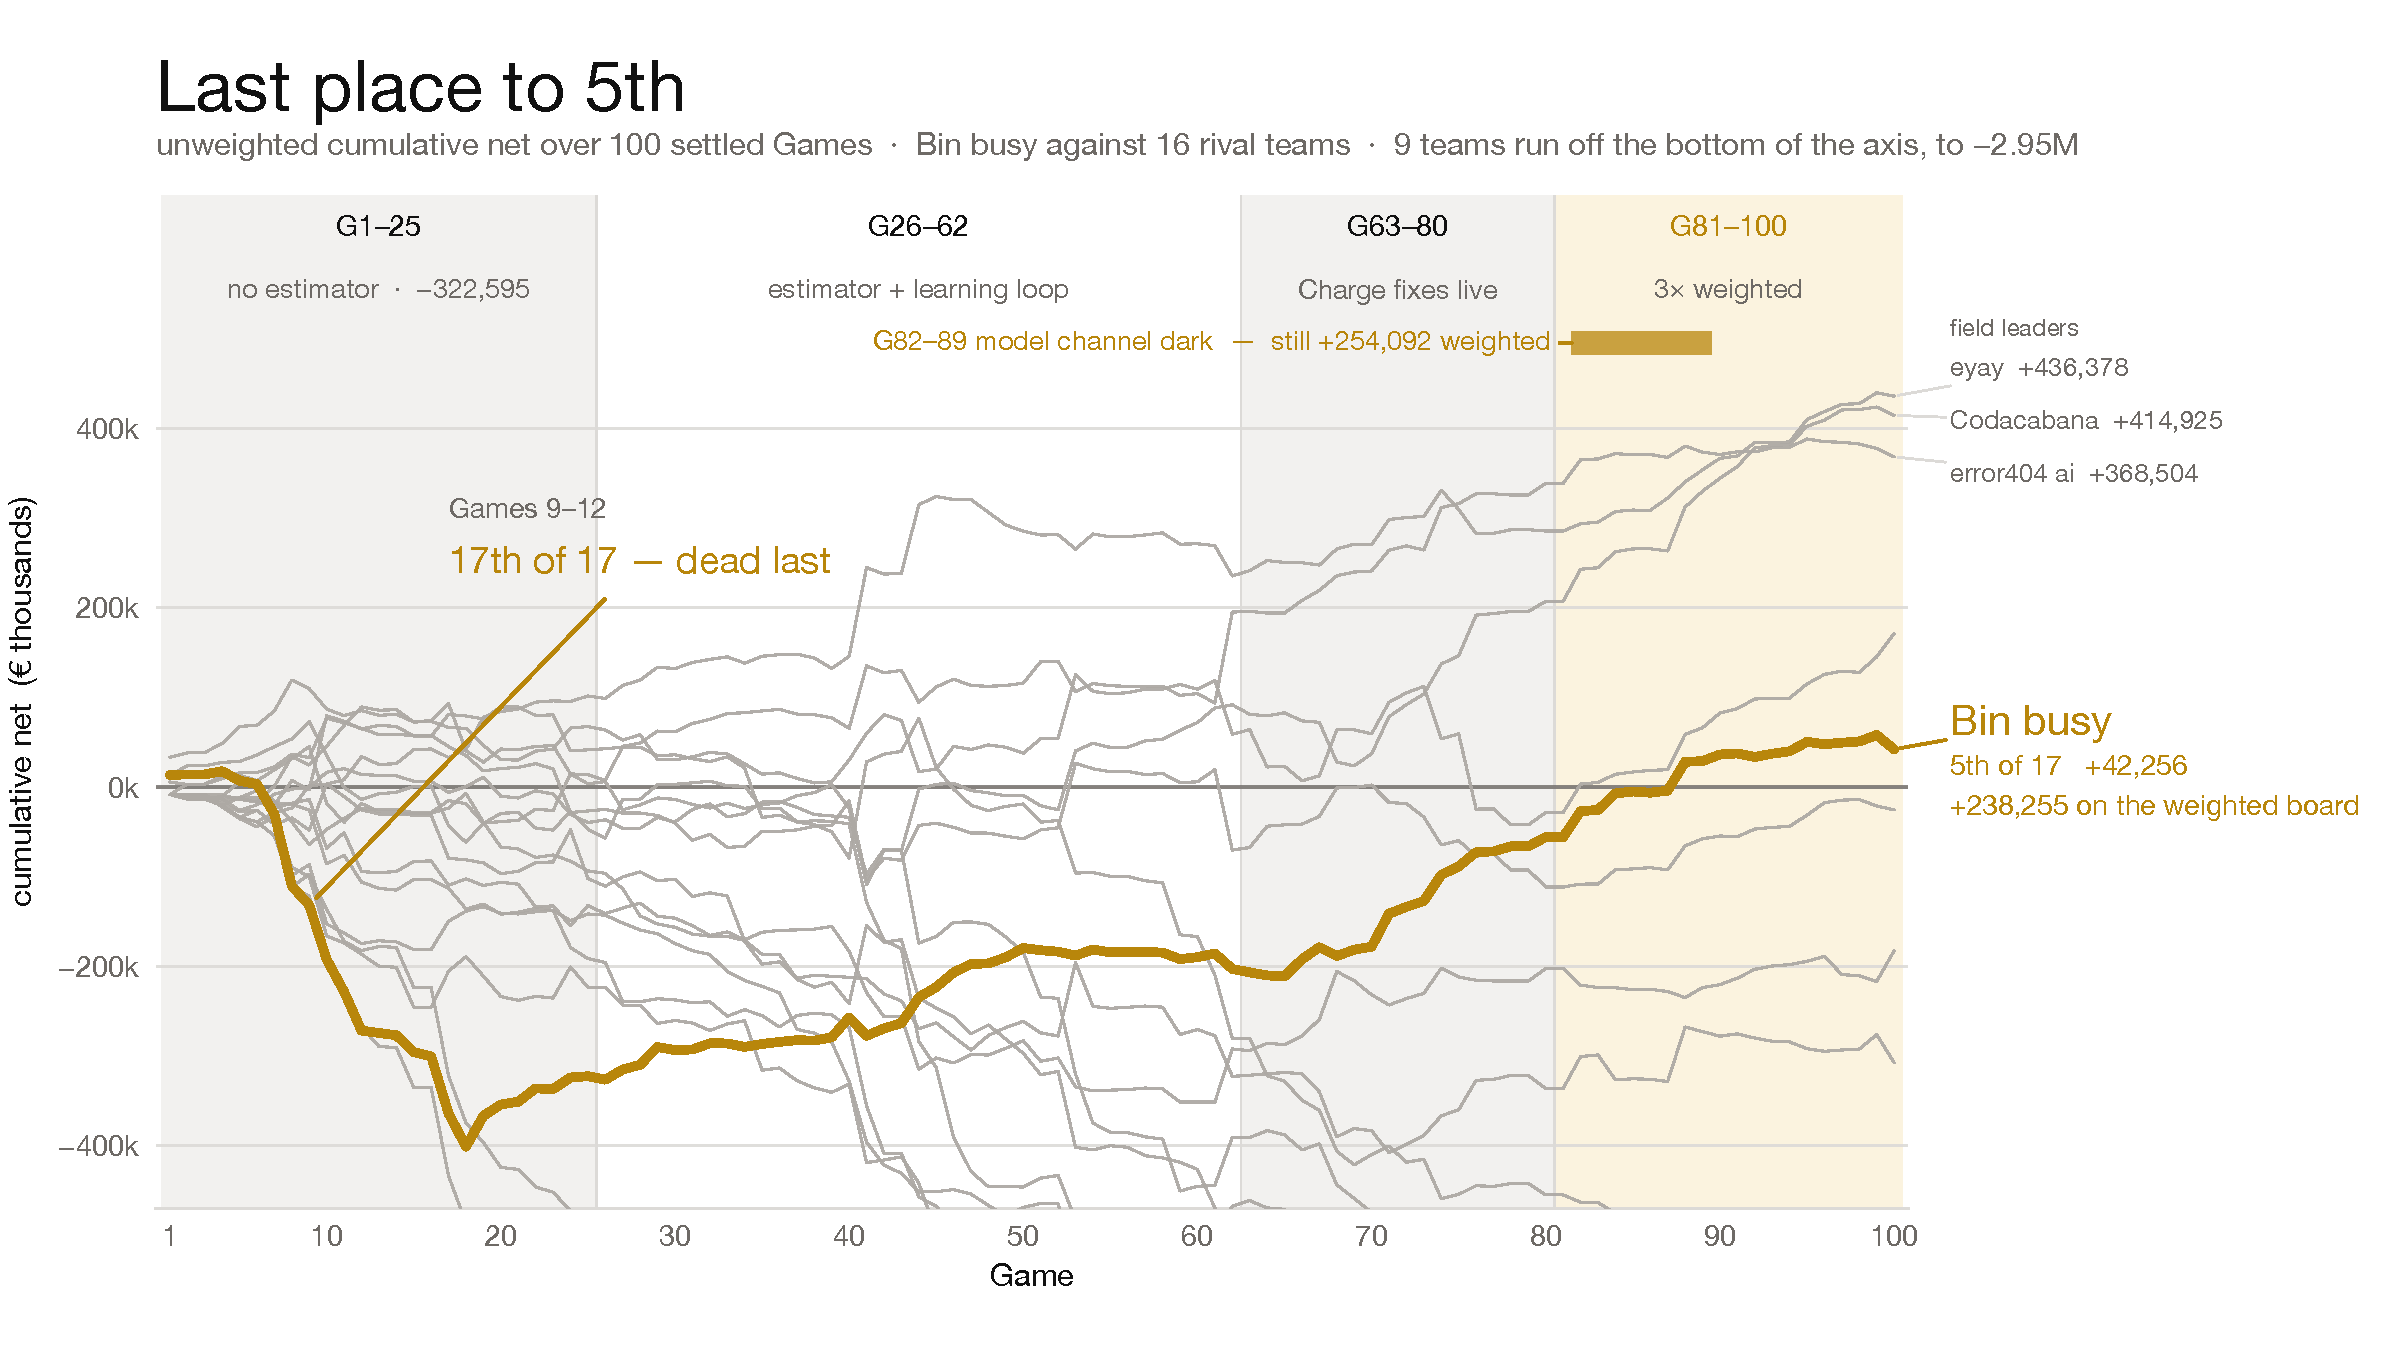
\includegraphics[width=\textwidth]{figures/balance-annotated-light.pdf}
\caption{Cumulative net over 94 settled Games, all 17 teams. We are the heavy line. The deficit is
Games 1--25, before the estimator existed; the slope after Game~26 is the method. Games 82--89 ran
with the model channel returning 401 on every call.}
\end{figure*}}{}

\onecolumn
\section*{\textcolor{accent}{Why we think we succeeded --- and where we did not}}
\vspace{-0.4em}
\begin{multicols}{2}
\subsection*{Succeeded}
\begin{itemize}
\item \textbf{We built the measuring instrument before the strategy.} Equation~\eqref{eq:inversion}
recovers $\fair$ exactly, so every later decision was settled by replaying it against the real
Field rather than argued. Three claims we had written down as fact were falsified within a day.
\item \textbf{Last place to 5\textsuperscript{th}.} 17\textsuperscript{th} of 17 after nine Games;
5\textsuperscript{th} from Game~76. Second in the field by rate over the last twenty Games; third
of seventeen over the 69 Games since the estimator existed, within $4.3\%$ of the leader.
\item \textbf{The distribution is tight, and that is the result we would defend.} Two losing Games
in the last twenty, the worst costing $3{,}941$; four in the last thirty, fewest of any team.
Mean-to-$\sigma$ of $0.72$, second best in the field, while five teams carry single Games worse
than $-80{,}000$. In an insurance book the narrow distribution is the number that matters.
\item \textbf{It degraded instead of failing.} Eight consecutive $3\times$-weighted Games ran with
the model channel completely dark and still banked $+254{,}092$, because no scored number ever
depended on a model being reachable.
\item \textbf{We priced uptime correctly.} Break-even uptime is $71\%$; rescuing a Game is worth
$93\fair$ against $37\fair$ for improving one, so \emph{showing up is 2.5$\times$ being right}. A
blind floor posts at T$+$0 before the Case is decrypted, submissions merge per Line Item, and a
supervisor restarts on any crash. Confirmed against a real opponent: \texttt{makalu} went dark,
paid us $179{,}993$ across the season and collected $0.00$ from anyone.
\end{itemize}

\subsection*{Did not succeed}
\begin{itemize}
\item \textbf{We spent the first quarter of the tournament building the instrument instead of
scoring.} Games 1--25 cost $-322{,}595$ --- more than our entire current season net. The rate says
the decision was right; the total says we paid full price for it.
\item \textbf{The estimate, not the strategy, is the whole remaining gap --- and we learned that
late.} $\charge=\limitv=\fair$ reaches $100.3\%$ of optimal play; $\charge=\limitv=\est$ scores
$-50{,}140$. The $2{,}498{,}118$ between them is pure estimation error. We tuned decision rules to
their measured argmax and it barely mattered; arguably we worked one layer too low.
\item \textbf{We diagnosed our largest open lever and deliberately did not ship it.} Policy clause
7.1.5 has two halves and the model reads only the first. Game~74 returned coverage $0.01$--$0.05$
on 20 of 31 Line Items, for $87\%$ of that Game's penalties. Perfect coverage is worth
$+1{,}173$/Game. It is a prompt change that could not be validated without spending the live
runner's quota, six Games before the $3\times$ window. We think the call was right and the outcome
is still a loss.
\item \textbf{Eight triple-weighted Games ran with the model dark and we did not notice.} It is the
best evidence we have that the architecture works, and simultaneously an operational failure: no
alert on \texttt{model\_draws=0}, during the most valuable Games of the tournament.
\item \textbf{We were beaten on the thing we understood best.} We had written down that the Charge
is a cliff and still sat above $\fair$ too often; a rival took $136{,}075$ off a single Line Item
by charging $22\%$ lower than us. Knowing a mechanism and being calibrated to it are different
achievements, and we only closed that gap at Game~63.
\end{itemize}
\end{multicols}

\vspace{0.6em}
\noindent\rule{\linewidth}{0.4pt}\\[0.3em]
{\footnotesize\textbf{No claim data is checked into this repository} --- not the Cases, the invoice
PDFs or the policies, and not the four derived paths that would reproduce them (raw model replies,
per-Game reviews, the submission-time decision log and the settled lessons all carry policy wording
or invoice Line Item text). All four regenerate locally and are git-ignored. Single-clause
quotations appear where the argument needs them, as citation rather than as an archive.
Every figure in this document is reproducible from a script in the repository.\par}


\end{document}
